%!TEX root = ../dokumentation.tex

%TODO: Einleitungen überarbeiten
\chapter{Concept}\label{cha:Concept}
This chapter outlines the concept and the architecture of the software tool. First, the proposed software architecture is described. Then the concept of each component is discussed.
 \section{Overview}\label{sec:ConceptOverview}
The software tool consists of five main components: the lexer, which extracts tokens from a \ac{TPTP} grammar file. The parser, which analyses the tokens and constructs a data structure representing the \ac{TPTP} grammar. todo

Figure \ref{fig:ConceptConceptWorkflow} outlines the main activities of the software tool in a 
\begin{figure}[H]
\tikzstyle{decision} = [ diamond, draw, fill=blue!10, text width=4.5em, text badly centered, node distance=2cm, inner sep-0pt]  
\tikzstyle{block} = [ rectangle, draw, fill=blue!10, text width=4.5em, text badly centered, rounded corners, minimum height=4em]  
\tikzstyle{line} = [ draw, -latex']  
%\tikzstyle{terminator} = [ draw, ellipse, fill=red!20, node distance=3cm, minimum height=2em]
\tikzstyle{terminator} = [rectangle, draw, fill=blue!10, text width=4.5em, text badly centered, rounded corners, minimum height=4em]  
\begin{center}
\begin{tikzpicture}[node distance=3cm, auto]  
  %\node [terminator]           (import)  {Import grammar file};  
  \node [terminator]           (import)  {Import of grammar file};
  \node [block, right of=import]  (lex)  {Lexing};  
  \node [block, right of=lex]  (pars) {Parsing};  
  \node [block, right of=pars] (ggg) {Grammar graph generation}; 
  \node [block, right of=ggg] (ggm) {Grammar graph modification}; 
    \node [block, right of=ggm] (go) {Grammar output};  
  \path [line] (import)  -- (lex);  
  \path [line] (lex)  -- (pars);  
  \path [line] (pars) -- (ggg);  
  \path [line] (ggg) -- (ggm); 
  \path [line] (ggm) -- (go);  
\end{tikzpicture}
\end{center}
\caption{General tool workflow}
\label{fig:ConceptConceptWorkflow}
\end{figure}

 \section{Requirements}\label{sec:ConceptRequirements}
The tool should meet the following requirements:\\
The tool has a GUI that is the interface between the tool and a user. Hence, the user communicates with the tool via the GUI. The user should be able to import a grammar file. After the grammar file is imported, the grammar file should be displayed. 
This includes displaying by the grammar defined productions as well as comments that are associated with grammar productions.
The user can select a new start symbol and can select which productions should be blocked. 
Productions can either be blocked as a whole or partly if the production is a disjunction.
After the user made his choice, the new reduced grammar should be generated and displayed.
The tool should also generate a control file listing blocked productions and the start symbol.
Furthermore, the tool should be able to import a control file and reduce a given grammar based on this control file instead of reducing a grammar based on a users selection of blocked productions.
The new reduced grammar should be exported to .txt format.
Also, comments referring to the remaining productions should be kept and comments referring to productions that fell away should not be included in the new grammar.
\subsection{Proposed Architecture}\label{sec:ConceptProposedArchitecture}

\section{Lexer}
The \ac{TPTP} language is specified in a modified \ac{EBNF}.
Therefore there are deviations from standard \ac{EBNF} (\ref{sec:BackgroundBNF}) that need to be analysed to specify elementary tokens in the lexer.
The standard \ac{EBNF} uses only only one production symbol ($"::="$).
In the \ac{TPTP} language additional production symbols have been added.
The following table \ref{tbl:ConceptTPTPProductionSymbols} contains the production symbols used in the \ac{TPTP} language.

\begin{table}[H]
\centering
\renewcommand{\arraystretch}{1}
\caption{\ac{TPTP} language production symbols \cite{VS06}}
\begin{tabular}{ll}
\textbf{Symbol} & \textbf{Rule Type}\\\hline
::= & Grammar\\
:== & Strict\\
::- & Token\\
::: & Macro\\
\end{tabular}
\label{tbl:ConceptTPTPProductionSymbols}
\end{table}

In the \ac{TPTP} language specification square brackets not necessarily denote that an expression is optional.
In token and macro rules they have the same meaning as in traditional  \ac{EBNF} and in grammar and semantic rules square brackets are terminals.
Also, there are line comments in the \ac{TPTP} language specification. A comment starts with the $\%$ symbol at the beginning of a line and ends at the end of this line.

\section{Parser}
\subsection{Data Structure}
The \ac{TPTP} grammar, extracted from the \ac{TPTP} grammar file, needs to be stored in a data structure that allows for modification. A graph representing
possible transitions within the 
\section{Generation of the Reduced Grammar}\label{sec:ConceptGenerateReducedGrammar}

\subsection{Selection of blocked Productions}

\subsection{Determination of the remaining reachable Productions}

\subsection{Determination of  the remaining terminating Productions}

\section{Maintainig Comments}\label{sec:ConceptMaintaining Comments}
In the \ac{TPTP} language specification there are comments providing supplemental information about the language and its symbols and rules.
When genering a  reduced grammar maintaining of comments is desired. This means that comments from the original language specification should be associated with the rule they belong to and if the rule is still present in the reduced grammar, also the comment should be.\\
Therefore a mechanism has to be designed for the association of comments to grammar rules.

\begin{lstlisting}[basicstyle=\scriptsize	,caption= Example of a comment in the \ac{TPTP} language specification,label= lst:ConceptComment_tptp]
%----Top of Page---------------------------------------------------------------
%----TFF formulae.
<tff_formula>          ::= <tff_logic_formula> | <tff_atom_typing> |
                           			  <tff_subtype> | <tfx_sequent>
\end{lstlisting}
heuristic:
comments near the rule the refer to
associate comment with r

bei tree building temporäres startsymbol nutzen (da mehrere Startsymbole möglich)

\begin{figure}[H]
\centering
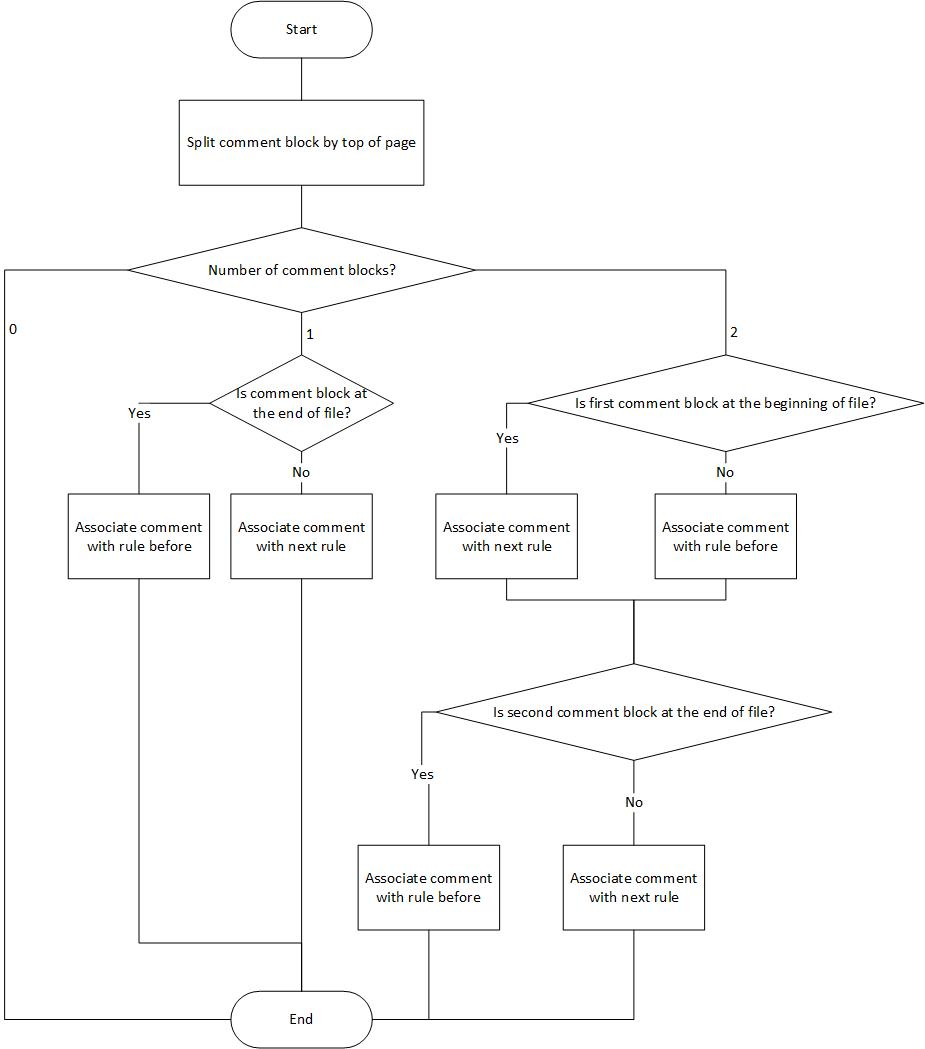
\includegraphics[width=1\textwidth]{images/maintainingComments.jpg}
\caption{Maintaining Comments}
\label{fig:comments}

\end{figure}

\section{Console Interface}\label{sec:Console Interface}

\section{GUI}\label{sec:ConceptGUI}


